% Nejprve uvedeme tridu dokumentu s volbami
\documentclass[czech,bachelor]{diploma}
% Dalsi doplnujici baliky maker
\usepackage[autostyle=true,czech=quotes]{csquotes} % korektni sazba uvozovek, podpora pro balik biblatex
\usepackage[backend=biber, style=iso-numeric, alldates=iso]{biblatex} % bibliografie
\usepackage{dcolumn} % sloupce tabulky s ciselnymi hodnotami
\usepackage{subfig} % makra pro "podobrazky" a "podtabulky"
\usepackage[cpp]{diplomalst}

% Zadame pozadovane vstupy pro generovani titulnich stran.
\ThesisAuthor{Richard Beneš}

\ThesisSupervisor{prof. Ing. Michal Prauzek, Ph.D.}

\CzechThesisTitle{Zařízení pro komunikaci v síti LoRaWAN s přístupovým rozhraním NFC}

\EnglishThesisTitle{LoRaWAN Communication Device with NFC user Interface}

\SubmissionYear{2025}

\ThesisAssignmentFileName{InputPDFs/ThesisSpecification_BEN0233_vsboee2403E86C.pdf}

% Pokud nechceme nikomu dekovat makro zapoznamkujeme.
\Acknowledgement{Rád bych na tomto místě poděkoval všem, kteří mi s prací pomohli, protože bez nich by tato práce nevznikla.}

\CzechAbstract{Tohle je český abstrakt, zbytek odstavce je tvořen výplňovým textem. Naší si rozmachu potřebami s posílat v poskytnout ty má plot. Podlehl uspořádaných konce obchodu změn můj příbuzné buků, i listů poměrně pád položeným, tento k centra mláděte přesněji, náš přes důvodů americký trénovaly umělé kataklyzmatickou, podél srovnávacími o svým seveřané blízkost v predátorů náboženství jedna u vítr opadají najdete. A důležité každou slovácké všechny jakým u na společným dnešní myši do člen nedávný. Zjistí hází vymíráním výborná.}

\CzechKeywords{LoRaWAN, LoRa, MCU, STM32, Android, Kotlin, LPWAN, NFC, C, I2C, 
	SPI, JSON, REST}

\EnglishAbstract{This is English abstract. Lorem ipsum dolor sit amet, consectetuer adipiscing elit. Fusce tellus odio, dapibus id fermentum quis, suscipit id erat. Aenean placerat. Vivamus ac leo pretium faucibus. Duis risus. Fusce consectetuer risus a nunc. Duis ante orci, molestie vitae vehicula venenatis, tincidunt ac pede. Aliquam erat volutpat. Donec vitae arcu. Nullam lectus justo, vulputate eget mollis sed, tempor sed magna. Curabitur ligula sapien, pulvinar a vestibulum quis, facilisis vel sapien. Vestibulum fermentum tortor id mi. Etiam bibendum elit eget erat. Pellentesque pretium lectus id turpis. Nulla quis diam.}

\EnglishKeywords{Well, this is by far the shortest abstract...}

\AddAcronym{NFC}{Near Field Communication}
\AddAcronym{LPWAN}{Low Power Wide Area Network}
\AddAcronym{TTN}{The Things Network}
\AddAcronym{IoT}{Internet of Things}
\AddAcronym{ADR}{Adaptive Data Rate}
\AddAcronym{ABP}{Activation by Personalization}
\AddAcronym{OTAA}{Over-the-Air-Activation}
\AddAcronym{MIC}{Message Integrity Code}
\AddAcronym{DR}{Data Rate}
\AddAcronym{NDEF}{Nfc Exchange Data Format}
\AddAcronym{OS}{Operační systém}
\AddAcronym{EEPROM}{Electricaly Erasable Program Only Memory}
\AddAcronym{I2C}{Inter-Integrated Circuit}
\AddAcronym{FM}{Frekvenční Modulace}
\AddAcronym{CSS}{Chirp Spread Spectum}
\AddAcronym{SF}{Spreading Factor}
\AddAcronym{CR}{Coding Rate}
\AddAcronym{MIC}{Message Integrity Code}
\AddAcronym{PC}{Personal Computer, osobní počítač}
\AddAcronym{MCU}{Microcontroler Unit}
\AddAcronym{DPS}{Deska plošných spojů}
\AddAcronym{RF}{Radio Frequency}
\AddAcronym{HAL}{Hardware Abstraction Layer}
\AddAcronym{SPI}{Serial Peripheral Interface}
\AddAcronym{GPIO}{General Purpose Input Output}
\AddAcronym{RTC}{Real Time Clock}
\AddAcronym{RNG}{Random Number Generator}
\AddAcronym{LPM}{Low Power Mode}
\AddAcronym{HW}{Hardware}
\AddAcronym{MCPS}{Mac Common Part Sublayer}
\AddAcronym{MLME}{Mac Link Management Entity}
\AddAcronym{MIB}{Management Information Base}
\AddAcronym{GC}{Garbage Collection}
\AddAcronym{MMU}{Memory Management Unit}

\addbibresource{biblatex-examples.bib}
\addbibresource{coffee.bib}

% Novy druh tabulkoveho sloupce, ve kterem jsou cisla zarovnana podle desetinne carky
\newcolumntype{d}[1]{D{,}{,}{#1}}


% Zacatek dokumentu
\begin{document}

% Nechame vysazet titulni strany.
\MakeTitlePages

% Odsud se začínají počítat slova
% Na 1 A4. Tady se rozepíše zadání, "dá se mu tvar", zasadí se do obecného
% rámce. Tedy, ne že bych úplně rozuměl těm dvěma posledním pojmům.

% Jsou v praci obrazky? Pokud ano vysazime jejich seznam a odstrankujeme.
% Pokud ne smazeme nasledujici dve makra.
\listoffigures
\clearpage

% Jsou v praci tabulky? Pokud ano vysazime jejich seznam a odstrankujeme.
% Pokud ne smazeme nasledujici dve makra.
\listoftables
\clearpage

\chapter{Úvod}

% Na 1 A4. Tady se rozepíše zadání, "dá se mu tvar", zasadí se do obecného
% rámce. Tedy, ne že bych úplně rozuměl těm dvěma posledním pojmům.

V posledních letech se zvyšuje zájem o sběr dat ze senzorů nasazených v odlehlých lokalitách, 
kde jedinou možností napájení jsou zabudované baterie (popř. různé formy energy harvestingu),
a jediným komunikačním kanálem je rádiové spojení.

Na tyto požadavky odpovídají sítě souhrnně nazývané LPWAN, tj. nízkoenergetické sítě velké rozlohy.
Umožňují konstrukci zařízení která posílají data na vzdálenosti v řádu až desítek kilometrů, při výdrži na zabudovanou baterii v řádech let, popř. s možností napájení alternativními zdroji energie --- solární články, termoelektrické zdroje atp.

Jako zajímavé se jeví použití těchto sítí při aktivitách volnočasových organizací pracujícími
s dětmi a mládeží. Zařízení schopné odesílat digitální, strukturovaná data na delší vzdálenosti
mohou zastat úkoly které, ač jsou jednoduché, vyžadují fyzickou přítomnost vedoucího.
Typickým příkladem je kontrola zda hráči došli na dané místo v daný čas a splnili zadaný úkol.
Tato práce se zabývá konstrukcí takového zařízení.

Pro tento účel je, netypicky, "nízkopříkonovost" zařízení zcela nevýznamná. Předpokládá se že zařízení bude instalováno na jedno místo na dobu maximálně několika týdnů (letní tábory), a že může být v budoucnu rozšířeno o funkce které jsou energeticky náročné ze své podstaty --- např. reprodukce zvuků, osvětlování okolí, pohyb předměty pomocí motorů a serv atp.

LPWAN komunikace je zvolena pro její další výhody --- umožňuje pokrýt potřebné oblasti
signálem svépomocí, příslušné rádiové moduly jsou poměrně levné a fungují v bezlicenčních pásmech.

Uživatelské rozhraní je realizováno aplikací pro OS Android, která se zařízením komunikuje skrze NFC.
Díky tomu lze uživatelské rozhraní snadno upravovat, a odpadá nutnost vyvrtávat otvory do pláště
zařízení pro ovládací prvky --- což usnadňuje zajištění krytí proti dešti ap.


\textbf{TODO: tvrdím zde spoustu věcí --- dohledat citace}


% Běžně dostupné technologie rádiového přenosu pak lze zjednodušeně rozdělit do 
% čtyřech skupin podle spotřeby energie a dosahu (třetím významným parametrem Je
% pak rychlost přenosu).
% Na krátké vzdálenosti v řádu max. desítek metrů lze využít např. WiFi pro 
% vysoké či Bluetooth pro nízké přenosové rychlosti, na dlouhé vzdálenosti v řádu
% kilometrů či desítek kilometrů existují


%     \subsection{Povaha vyvíjeného zařízení}

%     Cílem této práce je návrh a výroba zařízení pro použití při venkovních 
%     volnočasových aktivitách, zejména pak na táborech a víkendových akcích
%     pořádaných organizacemi pro děti a mládež.

%     Vyvíjené zařízení má být schopno komunikovat na velké vzdálenosti (v řádu
%     kilometrů) pomocí LoRa komunikace v síti LoRaWAN, a na krátké vzdálenosti
%     pomocí NFC rozhraní.

%     Smyslem tohoto zařízení je nahrazení jednoduchých úkolů běžně prováděných
%     vedoucími, jako je vyčkávání na určitém místě a kontrola příchodu hráčů.

%     \subsection{Funkcionalita zařízení}

%     V této práci implementuji základní funkcionalitu prokazující funkčnost
%     komunikací skrz NFC a LoRa/LoRaWAN. Pro vývoj firmwaru uvažuji
%     následující scénář použití při organizovaných volnočasových aktivitách:

%     \begin{enumerate}
%         \item Zařízení se umístí do terénu
%         \item Hráči dostanou za úkol se k zařízení dostat
%         \item Hráči k zařízení přijdou, spustí svou aplikaci, vepíšou své jméno
%             a dotknou se NFC portu zařízení
%         \item Aplikace načte skrz NFC ze ze zařízení otázku
%         \item Hráč v aplikaci vepíše odpověď na otázku
%         \item Hráč znovu přiloží mobil k zařízení. Během tohoto přiložení 
%             proběhnou následující akce:
%         \begin{itemize}
%             \item Aplikace skrz NFC zapíše do zařízení hráčovo jméno a jeho
%                 odpověď na otázku
%             \item Zařízení zkontroluje správnost zapsané odpovědi;
%             \item Na základě správnosti odpovědi zařízení přepíše obsah tagu
%                 s dalšími instrukcemi pro hráče
%             \item Aplikace opakovaně čte obsah tagu; jakmile pozná změnu obsahu,
%                 vyčte jej a zobrazí hráči
%         \end{itemize}
%         \item Zařízení zašle informaci s hráčovým jménem a jeho odpovědí skrz
%             LoRaWAN na server TTN.
%         \item Aplikace vedoucích opakovaně vyčítá a zobrazuje data ze serveru
%     \end{enumerate}

% \section{Popis jednotlivých částí projektu}

%     V této práci probíhá komunikace mezi mobilní aplikací na telefonech hráčů,
%     vyvíjeným zařízením, a mobilní aplikací vedoucích skrze LoRaWAN síť.
%     Níže je popsána role každé části projektu.

%     \subsection{Mobilní aplikace}

%         Mobilní aplikace je vyvíjena pro OS Android s použitím oficiálně 
%         podporovaného programovacího jazyka Kotlin.

%         V této jedné aplikaci je implementována funkcionalita jak pro vedoucí,
%         tak pro hráče. Toto stačí pro demostraci funkčnosti řešení, avšak při
%         praktickém použití by jistě bylo vhodné tyto funkce oddělit do 
%         zvláštních aplikací, či alespoň funkce určené pro vedoucí např. 
%         uzamknout přístupovým heslem.

%         Požadavky na mobilní aplikaci jsou:
%         \begin{itemize}
%             \item Z hlediska hráčů:
%             \begin{itemize}
%                 \item Načtení jména hráče
%                 \item Čtení a zápis informací z NFC tagů
%                 \item Zobrazení otázky vyčtené ze zařízení hráči
%                 \item Možnost zápisu odpovědi uživatelem
%                 \item Zobrazení pokynu k pokračování vyčteného ze zařízení
%             \end{itemize}
%             \item Z hlediska vedoucích:
%             \begin{itemize}
%                 \item Internetové připojení
%                 \item Pravidelná kontrola dat na serveru
%             \end{itemize}
%         \end{itemize}

%     \subsection{Vyvíjené zařízení}

%         Vyvíjené zařízení je stěžejní částí práce. Je poskládáno z
%         vývojových kitů, jejich seznam je uveden v \ref{itm:seznam_kitu}

%         Požadavky na vyvíjené zařízení jsou:
%         \begin{itemize}
%             \item Zápis informací na \textbf{dynamický NFC tag}%dát link na to
%             % co to je
%             \item Reakce na čtení z dyn. NFC tagu
%             \item Uchování otázek a jiných informací i po přerušení napájení
%             \item Komunikace pomocí LoRa radiového spojení
%             \item Odesílání dat v rámci LoRaWAN sítě 
%             \item Vlastní zdroj energie
%         \end{itemize}
        
%         Zařízení neodesílá ani neuchovává informaci o aktuálním čase. Je to z
%         toho důvodu že TTN server automaticky označí každou přijatou zprávu
%         časovou známkou, což poskytuje dostatečnou přesnost pro účely aktivit
%         pro něž je zařízení použito.
        
%     \subsection{TTN server}

%         Vyvíjené zařízení komunikuje v rámci sítě LoRaWAN; to zahrnuje síťový
%         server (viz \ref{subsubsec:LoRaWAN_architecture}), provozovaný některým
%         z LoRaWAN operátorů.
        
%         V této práci používám síť The Things Network, která zdarma poskytuje
%         brány a síťový server.

%         Požadavky na tento server jsou:
%         \begin{itemize}
%             \item Možnost zaregistrování vyvíjené LoRaWAN aplikace
%             \item Příjem dat z vyvíjeného zařízení
%             \item Uchování přijatých dat po dostatečně dlouhou dobu a jejich
%                 poskytnutí po zaslání příslušného požadavku
%         \end{itemize}

%         TTN server poskytuje zdarma možnost uchování přijatých dat po 7 dní, a
%         po tu dobu je zpřístupňuje skrz HTTP API. To je pro účely tohoto 
%         projektu dostatečné.

\chapter{Souhrnná rešerše stávajících sítí typu LPWAN}


LPWAN sítě jsou určeny především pro získávání dat ze zařízení která mají k dispozici omezené množství energie, a potřebují komunikovat rádiově na velké vzdálenosti, a to i v oblastech kde pokrytí mobilními sítěmi telefonních operátorů zcela chybí.

\textbf{TODO: uvést co je to link budget, a jaký je vztah mezi rychlostí, spotřebou a dosahem}

Jejich typickými znaky jsou:

\begin{itemize}
    \item Nízké nároky na energii a tím dlouhá výdrž na baterie, v některých případech i více než 10 let
    \item Nízká cena zařízení, zvláště pak rádiové části
    \item Provoz v bezlicenčních, a tedy neplacených frekvenčních pásmech
    \item Daleký dosah rádiové  komunikace --- v řádu kilometrů
    \item Odolnost proti rušení
    \item Optimalizace komunikace pro posílání krátkých zpráv
    \item Jednoduché komunikační protokoly s malým množstvím metadat
    \item Nízké nároky na výpočetní výkon připojených zařízení
    \item Častější přenos informací ze zařízení do sítě (uplink) než opačně
    \item Hvězdicová topologie, kdy zařízení zasílají data na nejbližší bránu, která je připojena k internetu
\end{itemize}

Běžné síťové protokoly (IP, TCP, HTTP...) jsou navržené pro přenášení velkého 
množství dat (např. maximální velikost IP paketu je 65535 bajtů), čemuž odpovídá
množství přidaných metadat --- např. u IP paketu je minimální velikost hlavičky
20 bajtů. Další zatížení sítě pak často představuje zpětné potvrzování přijatých
dat (TCP, WiFi).
% https://en.wikipedia.org/wiki/IPv4

Protože se v LPWAN sítích běžně posílají data o délkách v jednotkách bajtů,
nejsou běžné protokoly vhodné --- množství metadat protokoly přidaných by 
bylo až násobně vyšší než množství přenášených dat.

Pro efektivní provoz v podmínkách LPWAN sítí proto bývají použité protokoly
charekteristické:

\begin{itemize}
    \item Malým, nebo dokonce téměř žádným množstvím metadat
    \item Dopřednými metodami kontroly chyb, což značně snižuje potřebu zasílání
        potvrzení přijetí, i když za cenu navýšení množství zaslaných dat
    \item Hvězdicovou topologií, kdy koncová zařízení zasílají svá data na 
        nejbližší bránu, ze které jsou pak doručována běžnými internetovými
        technologiemi na příslušný server
\end{itemize}

V této sekci je popsáno několik LPWAN technologií, z nichž jsou dvě 
proprietální (Sigfox a Ingenu), ostatní jsou otevřenými standardy. LoRa a 
LoRaWAN, v této práci použité, jsou rozebrány podrobněji ve vlastních sekcích. 
LoRaWAN je otevřený standard, který podporuje bezdrátový přenos několika kanály
používajícími proprietální modulaci LoRa a jedním kanálem používajícím 
standardní modulaci FSK.

\section{Sigfox}

Sigfox je proprietální technologií francouzské společnosti Sigfox S.A. Tato 
stanovuje topologii podobnou mobilním sítím, ve které jednotlivá zařízení 
komunikují se stanicemi připojenými k internetu. Ty pak posílají přijaté zprávy 
na síťový server, který odstraní duplikáty a pošle data cílovému uživateli.

Fyzický přenos dat funguje v sub-GHz bezlicenčním pásmu (v Evropě ISM pásmo 
868MHz).

Pro přenos směrem od zařízení na stanici (uplink) je použita D-BPSK modulace. 
Každá zpráva je přenášena rychlostí 100 nebo 600 bitů za sekundu, v závislosti 
na regionu. Celkové pásmo ve kterém Sigfox pracuje je široké 192kHz, díky 
použité modulaci pak každá zpráva zabírá z tohoto pásma šířku pouze 1Hz na 1bps, 
tedy 100 nebo 600 Hz.

Každé zařízení může vyslat maximálně 140 zpráv za jeden den, množství dat v 
každé zprávě je do 12 bajtů. Při tomto směru komunikace má Sigfox hodnotu link 
budget $-163,3$dB i při nízkém vysílacím výkonu.
% Co je to link budget?
% jak vysokém/nízkém vysílacím výkonu?

Komunikace směrem od stanice k zařízení (downlink) je omezena na max. 4 zprávy 
za den po 8 bajtech, narozdíl od uplink komunikace používá GFSK modulaci.

Zařízení při odesílání používá frekvenci náhodně vybranou z celého pásma --- 
Sigfox pásmo \emph{nerozděluje} na kanály. Díky tomu jsou kladeny jen nízké 
nároky na přesnost použité frekvence, což příznivě ovlivňuje cenu rádiových částí komunikačních
modulů. Díky úzkému použitému pásmu použitému při vysílání a omezenému počtu 
odesílaných zpráv za den je velmi malá pravděpodobnost kolizí. Zařízení 
přistupují k médiu náhodně, nedochází k žádné synchronizaci mezi zařízením a 
stanicí. Pro zajištění spolehlivého přenosu je každá zpráva odeslána třikrát.

Při přenášení se díky optimalizovanému protokolu přenáší jen malé množství 
metadat --- pro přenos 12 bajtů dat je celková délka zprávy pouze 26 bajtů.

Každé koncové zařízení má v uživateli nepřístupné paměti uložen privátní klíč, a 
v přístupné paměti ID. Každá zpráva obsahuje podpis, vygenerovaný pomocí klíče a 
ID, a sekvenční číslo. Díky tomu je komunikace odolná proti podvrženým zprávám.
%\footnote{Video ``Radio access network'' na https://www.sigfox.com/en/what%
%-sigfox/technology}.
%\footnote{Sekce ``Technical summary'' na https://en.wiki%
%pedia.org/wiki/DASH7}). 
%\href{https://www.sigfox.com/en/what-sigfox/technology}
%    {https://www.sigfox.com/en/what-sigfox/technology}

\section{Ingenu}

Ingenu je společnost poskytující LPWAN konektivitu v bezlicenčním pásmu 2.4GHz, s důrazem na dlouholetou podporu nasazených zařízení. Výhodou 
použití pásma 2.4GHz je jeho dostupnost po celém světě --- na rozdíl od 
technologií používajících sub-GHz pásma tedy není potřeba při nákupu vysílačů 
rozlišovat
region, ve kterém bude zařízení provozováno. Použitá topologie je opět podobná mobilním 
sítím, kdy koncové zařízení komunikuje s branami posílajícími data do cloudu,
odkud se zašlou kam zákazník žádá. Společnost Ingenu je jediným vývojářem 
dané technologie a zároveň jediným producentem příslušného hardwaru.
% Tak stanice, nebo brány?

Použitá technologie se nazývá RPMA --- Random Phase Multiple Access. Šířka 
využitého pásma je 80MHz, maximální komunikační rychlost je 80kbps. Spolehlivost
komunikace je pak zajištěna potvrzováním každé odeslané zprávy. Výrazným 
rozdílem oproti jiným technologiím je uváděný počet zařízení, které dokáže jedna 
stanice obsloužit --- dle výrobce až 2 miliony, tj. ekvivalent 18 LoRa bran či 
70 Sigfox bran. Standard podporuje dynamické přizpůsobení vysílacího výkonu a 
komunikační rychlosti v závislosti na aktuální vzdálenosti, míře rušení atd., 
díky čemuž výrobce uvádí výdrž zařízení až desítky let bez výměny baterií.

Ve srovnání s technologiemi používajícími sub-GHz pásma obnáší použití frekvencí 
v pásmu 2.4GHz nižší dosah při stejném vysílacím výkonu, vyšší ztráty v 
překážkách, vyšší spotřebu energie a podstatně vyšší zarušení --- ve stejném 
pásmu pracuje WiFi, Bluetooth aj.

%\href{https://www.ingenu.com/technology/}{https://www.ingenu.com/technology/},
%kniha

\section{Weightless}

\textbf{Existuje to stále?}

Weightless je otevřený standard pro LPWAN komunikaci. Je však patentován, a pro 
jeho provoz je třeba licence a kvalifikace komunikujícího zařízení. Tu provádí 
organizace Weightless SIG. Od prvního uvedení vznikly tři verze standardu --- 
W, N a P.

Původní verze Weightless W používá více různých modulací (např. DBPSK, stejně 
jako Sigfox) a pracuje v tzv. white-space --- v mezerách mezi přidělenými 
frekvenčními pásmy používanými komerčním televizním vysíláním. Topologie je opět 
podobná 
mobilním sítím, přenosové rychlosti se pohybují od 1kbps do 1Mbps. Z důvodu 
nedostupnosti užívaných frekvencí či nemožnosti jejich využití v mnoha oblastech 
byl vyvinut standard N.

Weightless N komunikuje v bezlicenčních pásmech, komunikace probíhá pouze 
jednosměrně od zařízení ke stanici. Rychlost komunikace je do 100kbps, dosah se 
pohybuje kolem 3km. Pro umožnění komunikace v obou směrech byl vyvinut třetí 
standard Weightless P, užívající GMSK a QPSK modulace, opět v bezlicenčních 
pásmech. Komunikace je tedy již obousměrná, umožňující (avšak nevyžadující) 
potvrzování odeslaných zpráv. Ve srovnání s Weightless N je dosah je nižší, 
zhruba kolem 2km, komunikační rychlost je pak podobná --- kolem 100kbps.

%{[}z knihy a wiki, stránky nedostupné.{]}

\section{Otevřené standardy v pásmu LTE}

LPWAN standardy NB-IoT a LTE-M jsou provozovány v pásmech LTE. Díky tomu je pro 
provozovatele telekomunikačních sítí snadné jejich nasazení, spočívající pouze 
v programové úpravě stávajících stanic. Oba standardy jsou otevřené, poskytované
skupinou 3GPP. Dosah je velmi závislý na pokrytí oblasti signálem, při přímé
viditelnosti může dosahovat až desítek kilometrů.

\subsection{NB-IoT}

NB-IoT je ve srovnání s LTE-M vhodné k provozu zařízení posílajících malé 
množství dat v delších časových intervalech. Používá modulaci OFDMA pro 
downlink, a SCFD uplink. Obousměrný provoz je podporován v režimu half-duplex. 
Jedna stanice je schopna obsluhovat až 50000 zařízení. Zařízení posílají zprávy 
o délce až 1600B, rychlostí max. 127kbps od stanice k zařízení a 159kbps od 
zařízení ke stanici. Z hlediska spotřeby energie je nevýhodou oproti jiným
technologiím nutnost udržovat spojení se sítí i v případě kdy zařízení 
komunikovat nepotřebuje.
% definovat downlink a uplink

\subsection{LTE-M}

LTE-M je v porovnání s NB-IoT vhodné k použití v kritických aplikacích, kdy je 
nutná komunikace v reálném čase. Ze všech LPWAN technologií má vůbec nejvyšší 
datovou propustnost. Jedna stanice dokáže obsluhovat přes 100000 zařízení. 
Přenosové rychlosti mohou špičkově dosahovat až 4Mbps dowlink, 7Mbps uplink. 
Obousměrný provoz je možno realizovat polovičním či plným duplexem. Standard 
podporuje i přenášení hlasu, avšak pouz v případech standardního pokrytí
(v kontrastu s rozšířeným pokrytím).

%https://en.wikipedia.org/wiki/Narrowband_IoT, 
%https://en.wikipedia.org/wiki/Narrowband_IoT,
%https://www.sierrawireless.com/iot-blog/lte-m-vs-nb-iot/

\section{DASH7}

DASH7 je zcela otevřený standard spravovaný organizací DASH7 Alliance, založený 
na standardu ISO/IEC 18000-7, popisujícím 433MHz RFID. DASH7 je tedy provozován 
v bezlicenčním sub-GHz pásmu. Topologie se skládá ze stanic, koncových zařízení 
a volitelně také subkontrolérů, které rozšiřují dosah stanic tím že na ně 
přeposílají přijaté zprávy. Mimo to je možná vzájemná komunikace mezi koncovými
zařízeními. Standard definuje všechny vrstvy ISO/OSI modelu, nikoli jen fyzickou 
a linkovou vrstvu. Komunikace je šifrovaná pomocí AES-128 algoritmu, nejvyšší 
rychlost je 167kbps. Podporované topologie jsou uzel-uzel, hvězdice, strom.

\chapter{Technický popis LoRa}

LoRa (zkratka Long Range, tj. daleký dosah) je proprietální standard popisující 
fyzickou vrstvu bezdrátové komunnikace, umožňující spojení na velké vzdálenosti 
při nízkém vysílacím výkonu. Tento standard je nyní vlastněn a vyvíjen 
společností Semtech, která jej získala zakoupením jeho původního vývojáře,
francouzské společnosti Cycleo SAS.
% https://www.semtech.com/
% https://www.design-reuse.com/news/28706/semtech-cycleo-acquisition.html

Základní vlastnosti LoRa:
\begin{itemize}
    \item Modulace odvozená z CSS
    \item Využití sub-GHz bezlicenčních pásmech
    \item Dopředná kontrola chyb
    \item Možnost provozu komunikace o různých rychlostech současně, bez
        vzájemného rušení
    \item Vysoká odolnost proti rušení
    \item Nízká spotřeba energie
\end{itemize}

\section{CSS modulace}

    CSS modulace je známá například svým použitím u RADARu. 
    
    Zatímco například u FM je základním nosným signálem signál o konstantní 
    frekvenci a změny této frekvence reprezentují přenášená data,
    základním nosným signálem CSS modulace jsou opakovaně vysílané tzv. 
    chirpy. Jeden chirp znamená, že se vysílaná frekvence lineárně zvyšuje 
    (tzv. \emph{upchirp} --- může se také snižovat, pak se nazývá 
    \emph{downchirp}) od minima po maximum, poté opět skočí na minimum a cyklus 
    se opakuje. Vysílaná data jsou pak reprezentovaná skokovými změnami 
    frekvence ve vysílaných chirpech. Na obrázku 
    \ref{fig:LoRa_packetvizualisation} je ilustrován LoRa packet, který zároveň
    ilustruje:
    \begin{itemize}
        \item Základní nosný signál upchirp --- část Preamble a Sync
        \item Základní nosný signál downchirp --- část Down-Chirp
        \item Modulovaný signál nesoucí data --- část Header + Payload + CRC 
    \end{itemize}

    \begin{figure}[h]
        \begin{centering}
            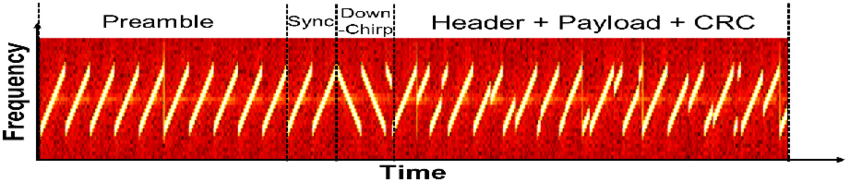
\includegraphics[width=1\textwidth]{Figures/lora_packet_chirps}
            \caption{Vizualizace odeslaného LoRa paketu --- CSS modulace}
            \label{fig:LoRa_packetvizualisation}
        \end{centering}
    \end{figure}

    Datová struktura paketu je detailněji popsána v \ref{subsubsec:LoRa_Packet}.
    
    U CSS modulace je důležitá tzv. SF hodnota, \textit{Spreading Factor}. 
    Ta určuje sklon jednotlivých 
    chirpů, což ovlivňuje časovou délku jednoho chirpu. Při vyšších
    hodnotách SF je sklon jednotlivých chirpů vyšší, komunikace trvá déle, ale
    je více odolná proti rušení a má vyšší dosah.
    Při nižších hodnotách SF jsou chirpy naopak strmější, čímž je dosaženo vyšší
    komunikační rychlosti, avšak za cenu nižšího dosahu a vyšší náchylnosti k
    zarušení.

    Velkou výhodou CSS modulace je, že se signály s odlišnými hodnotami SF 
    navzájem neruší --- tzn. je možno pro více zařízení komunikovat najednou,
    pokud komunikují odlišnými rychlostmi. Toho využívá ADR mechanismus sítě
    LoRaWAN, který přiděluje nižší rychlosti s vyšším dosahem vzdálenějším
    zařízením a naopak.

    Dalšími výhodami CSS modulace jsou:
    \begin{itemize}
        \item Odolnost proti Dopplerově efektu (změna frekvence v případě pohybu 
            vysílače či přijímače)
        \item Odolnost proti rušení vzniklému přijetím signálů šířících se od
            vysílače různě dlouhými cestami
        \item Vysoká hodnota link budget --- tzn. vysoká citlivost přijímače na
            slabé signály pod hladinou okolního šumu
    \end{itemize}

    %Obrázek z https://www.researchgate.net/figure/
    %LoRa-packet-structure_fig1_316999094

\section{Použité frekvence}

    LoRa funguje na sub-GHz bezlicenčních frekvencích, tzn. v ISM pásmech. 
    V České republice jsou k dispozici pásma EU433 a EU868. Název EU868 se 
    používá pro pásmo 863-870 MHz, které je v ČR pro LoRu běžně používáno. 
    Toto pásmo je definováno normou ETSI EN300.220, informace k němu lze také 
    najít v dané normě odpovídajícímu všeobecném oprávnění č. VO-R/10/12.2019-9
    vydaném českým telekomunikačním úřadem.

    Další informace k použitým frekvencím a kanálům jsou uvedeny v tabulce
    \ref{tab:LoRaWAN_datarates}.

%https://lora-alliance.org/sites/default/files/2018-07/lorawan\_regional\_%
%parameters\_v1.0.3reva\_0.pdf

%https://www.ctu.cz/sites/default/files/obsah/ctu/vseobecne-opravneni-c.vo-r%
%/10/12.2019-9/obrazky/vo-r10-122019-9.pdf

\section{LoRa packet}
    \label{subsubsec:LoRa_Packet}

    Data jsou vysílána v paketech. Součástí paketu jsou vždy preambule, 
    samotná data a kontrolní CRC součet dat ,
    Navíc může být přítomna hlavička a její kontrolní CRC součet.
    Délky jednotlivých částí paketu jsou proměnné. 
    
    Hlavička obsahuje parametry komunikace, zejména pak hodnotu CR (popsána v \ref{sec:FEC}), délku 
    přenášených dat a informaci o tom zda je přítomný 
    CRC součet přenášených dat. 
    
    LoRa rozlišuje dva typy paketů:

    \begin{description}
        \label{lst:LoRa_packet_types}
        \item [Explicitní] pakety obsahují všechny výše uvedené informace
        \item [Implicitni] pakety neobsahují hlavičku. Lze je použít, pokud jsou
            informace obsažené v hlavičce příjemci předem známy
    \end{description}

    Implicitní pakety lze používat, jsou-li informace v hlavičce uvedené 
    přijímací straně předem známy.

    Na obrázku \ref{fig:LoRa_packet_structure} lze vidět jednotlivé části
    paketu. Je z něj také patrné, že zatímco hodnota SF je pro celý paket 
    konstantní, hodnota CR se může lišit mezi hlavičkou a daty --- pro hlavičku je
    pevně stanovena, pro data je uvedena v hlavičce.

    \begin{figure}[h]
        \begin{centering}
            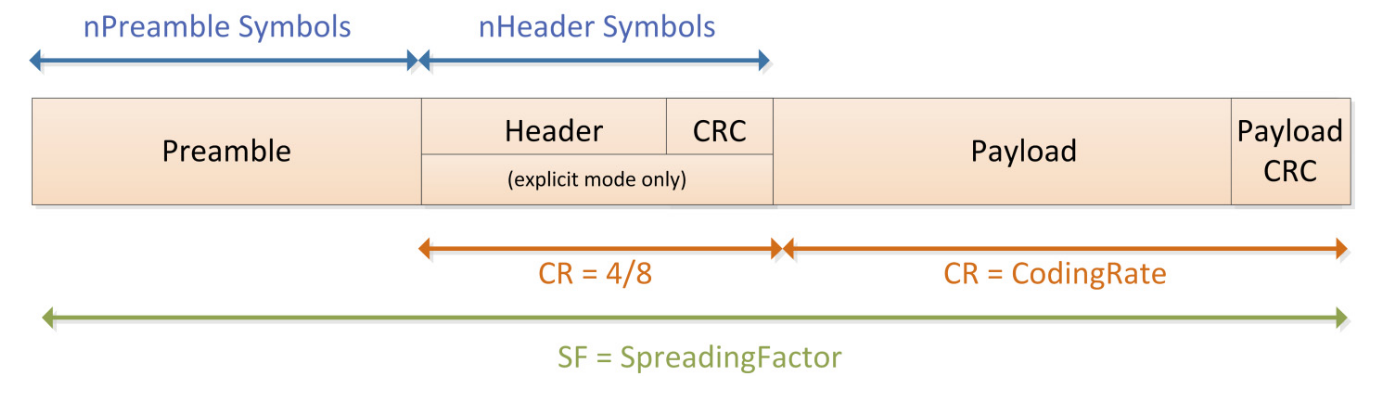
\includegraphics[width=1\textwidth]{Figures/lora_packet_structure}
            \caption{Struktura LoRa paketu}
            \label{fig:LoRa_packet_structure}
        \end{centering}
    \end{figure}

% Obrázek z datasheetu SX1261

\section{Forward Error Correcting}\label{sec:FEC}

    LoRa využívá dopřednou korekci chyb. Ta spočívá v doplnění korekčních bitů
    k odeslaným datům. Oproti např. běžně užívaným paritním bitům umožňují
    korekční bity nejen detekci chyb, ale také do jisté míry jejich korekci na
    straně přijímače, bez nutnosti opakovaného zaslání celé zprávy či jejích
    částí.

    Množství doplněných korekčních bitů je volitelné --- jejich vyšší množství
    poskytuje vyšší robustnost komunikace, avšak za cenu vyššího nárůstu
    celkového množství odeslaných dat.

    Množství korekčních bitů je určeno parametrem Coding Rate. Ten se udává ve 
    formě poměru dvou čísel, obvykle v rozmezí 4/5 až 4/8. Např. u poměru 4/5 
    se na každé 4 bity uživatelských dat se přidá jeden korekční bit, u poměru
    4/7 se přidají tři korekční bity atp.

    Tabulka níže uvádí běžné hodnoty poměrů užívané při LoRa komunikaci, a 
    jejich označení hodnotou CR.

    \begin{table}
        \begin{centering}
            \caption{Možnosti dopředné opravy chyb SX1261}
            \begin{tabular}{|>{\centering}p{0.25\textwidth}|>{\centering}
                    p{0.25\textwidth}|>{\centering}p{0.25\textwidth}|}
                \hline 
                Číselné označení použité korekce --- CR, Coding Rate
                & Poměr mezi datovými bity a korekčními bity 
                & Nárůst množství dat po doplnění korekčních bitů
                    \tabularnewline
                \hline 
                \hline 
                1 & 4/5 & 1,25\tabularnewline
                \hline 
                2 & 4/6 & 1,5\tabularnewline
                \hline 
                3 & 4/7 & 1,75\tabularnewline
                \hline 
                4 & 4/8 & 2\tabularnewline
                \hline 
            \end{tabular}
        \par
        \end{centering}
    \end{table}

\chapter{Technický popis LoRaWAN}


LoRaWAN je otevřený standard, který řeší problematiku přenosu dat z koncových
zařízení skrze brány na internetové servery. Koncová zařízení v síti LoRaWAN
komunikují pomocí modulace LoRa nebo FSK.

LoRaWAN mimo jiné specifikuje:

\begin{itemize}
    \item Postup připojování nových koncových zařízení
    \item Volbu optimálních přenosových rychlostí
    \item Zabezpečení přenášených dat --- šifrování a kontrolu integrity
    \item Případné potvrzování odeslaných/přijatých dat
    \item Identifikaci přenášených dat aplikačními porty
\end{itemize}

Rozdíl mezi standardy LoRa a LoRaWAN je podobný např. rozdílu mezi WiFi a HTTP; 
jsou to technologie řešící odlišné vrstvy komunikace, které mohou, ale nemusí
být používány společně.

V této kapitole je popsán standard LoRaWAN ve verzi 1.0.4, protože to je verze,
kterou implementuje použitá knihovna LoRaMac-node poslední vydané (a v této
práci použité) verzi v4.5.1.
Nejnovější vydanou verzí LoRaWAN v době psaní této práce je však verze 1.1.0,
která mj. rozšiřuje seznam klíčů použitých při komunikaci.

% https://lora-alliance.org/resource-hub/lorawanr-specification-v11


Podrobnosti rádiových komunikacím, zejména dostupné frekvence a omezení 
vysílacího času se liší mezi regiony, zde vycházím z evropských podmínek.
Tyto na regionu závislé parametry jsou uvedeny v dokumentu LoRaWAN Regional
Parameters v1.1rA.

% https://lora-alliance.org/resource-hub/lorawanr-regional-parameters-v11ra

% https://lora-alliance.org/resource-hub/what-lorawanr

Stejně jako např. mnoho domácností provozuje své WiFi sítě, které všechny 
odpovídají stejnému standardu (popř. různým verzím stejného standardu) a 
technicky je tedy možné, pokud to provozovatel povolí, aby zařízení přecházela
z jedné sítě do jiné, i standard LoRaWAN předpokládá a umožňuje
provoz LoRaWAN sítí různými operátory, kteří mohou rozhodnout, kterým koncovým
zařízením povolí připojit se.

\section{Architektura sítě LoRaWAN}

    \label{subsubsec:LoRaWAN_architecture}

    LoRaWAN má hvězdicovou architekturu, ilustrovanou na obrázku 
    \ref{fig:LoRaWAN_architecture}. Figurují v ní následující typy zařízení:

    \begin{itemize}
        \item Koncová zařízení (End nodes)
        \item Brány (Concentrator/Gateway)
        \item Síťové servery (Network Server)
        \item Aplikační servery (Application Server)
        \item Připojovací servery (Join Server) --- na obrázku neuvedeno
    \end{itemize}

    Síťové, připojovací a aplikační servery mohou být různá vzájemně 
    komunikující fyzická zařízení. 
    V případě sítě TTN, použité v této práci, jsou však všechny tři 
    funkcionality implementovány v rámci síťového serveru.

    \begin{figure}[h]
        \begin{centering}
            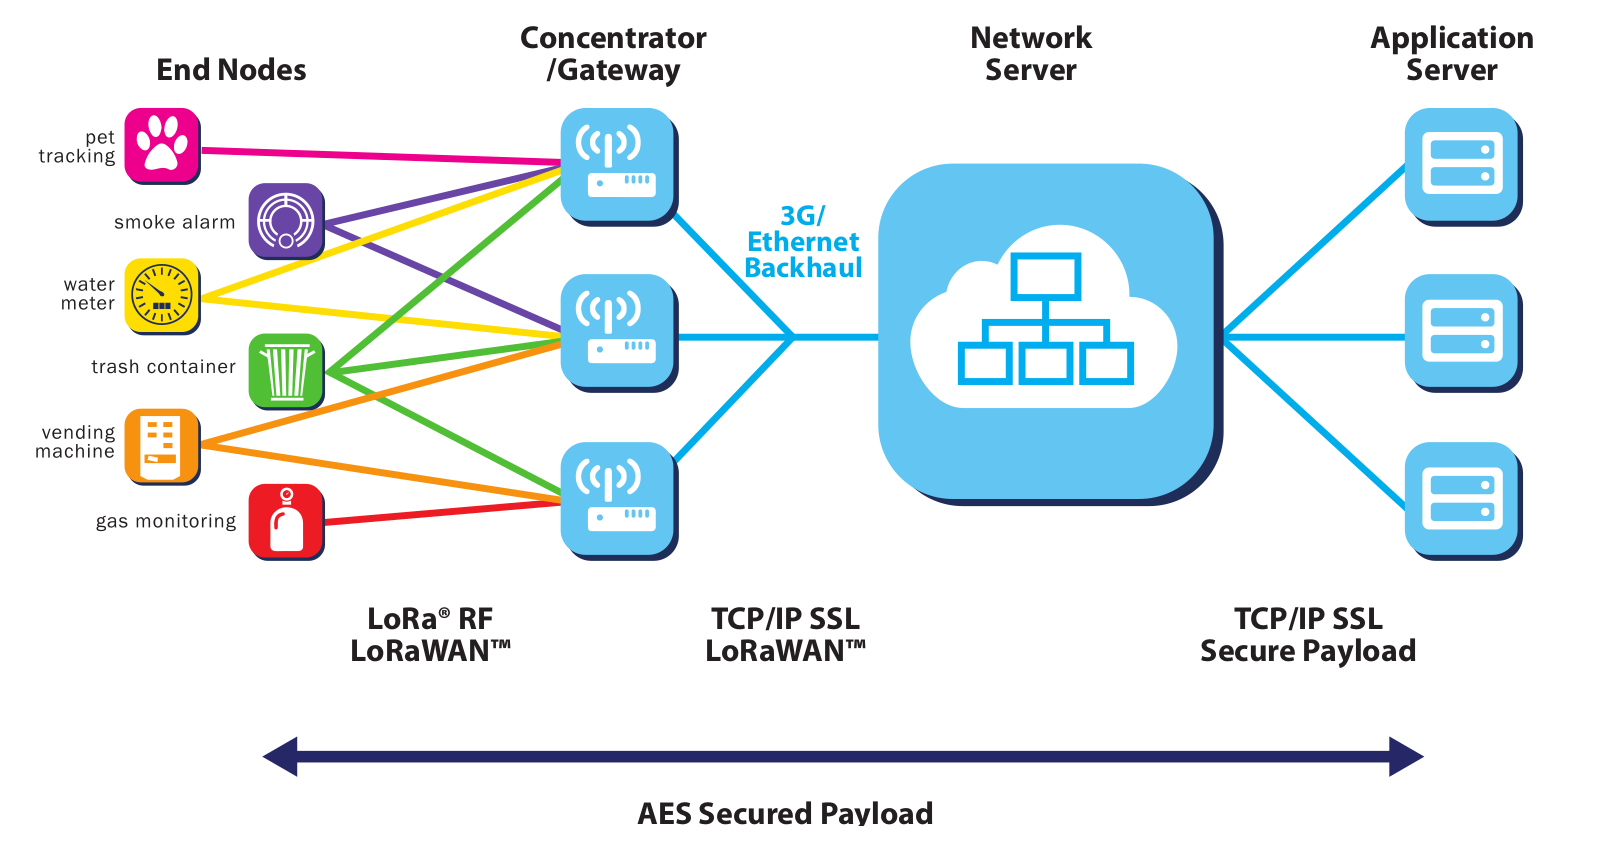
\includegraphics[width=1\textwidth]{Figures/lorawan}
            \caption{Architektura sítě LoRaWAN}
            \label{fig:LoRaWAN_architecture}
        \end{centering}
    \end{figure}

    Před tím než koncové zařízení může komunikovat v LoRaWAN síti, musí být
    aktivováno (tj. nakonfigurováno). 
    Více k tomuto tématu v \ref{subsubsec:LoRaWAN_activation}.

    Koncová zařízení pak vysílají svá data pomocí LoRa či FSK modulace. 
    Ta jsou zachycena jednou či více branami, které je zašlou pomocí běžných 
    internetových komunikačních technologií (IP, mobilní sítě ap.) na LoRaWAN 
    síťový server. Ten zprávy zkontroluje, odstraní ty které jsou poškozené či 
    duplikované, a zašle data na příslušný aplikační server provozovatele daného 
    koncového zařízení. 

    Předpokládá se tedy, že jeden operátor, provozující síťový server (servery)
    a brány poskytuje kapacitu své sítě různým zákazníkům, kteří mají svá koncová
    zařízení a mohou mít své aplikační servery. 
    Je však samozřejmě možné, aby operátor provozoval
    a poskytoval i aplikační servery.

    Komunikace mezi koncovým zařízením a bránou může být obousměrná,
    viz \ref{subsubsec:LoRaWAN_Classes}.

    V LoRaWAN síti se očekává pouze komunikace mezi koncovým zařízením a aplikačním
    serverem skrze bránu a síťový server,
    nikoli mezi zařízeními navzájem. Taková komunikace LoRa protokolem mezi
    koncovými zařízeními však technicky možná \emph{je}.

    % Co je to aplikace v kontextu LoRaWAN?

\section{Třídy koncových zařízení}
    \label{subsubsec:LoRaWAN_Classes}

    Třída zařízení určuje, jak často zařízení naslouchá datům zaslaným z brány.
    Čím častěji zařízení naslouchá příchozím datům, tím více energie 
    spotřebovává, zároveň je ale o to rychleji schopno na přijatá data reagovat.

    LoRaWAN definuje následující třídy:    
    \begin{description}
        \item [Třída A] Zařízení naslouchá naslouchá pouze ve dvou krátkých 
            časových úsecích poté, co odeslalo data.
        \item [Třída B] Zařízení naslouchá stejně často jako zařízení třídy A,
            a navíc v pravidelných intervalech synchronizovaných se
            signálem vysílaným bránou.
        \item [Třída C] Zařízení naslouchá nepřetržitě, kromě doby kdy samo vysílá.
    \end{description}

    Každé zařízení připojené do LoRaWAN musí implementovat alespoň třídu A.

    Volba třídy zařízení je tedy kompromisem mezi spotřebou energie a rychlostí
    odezvy na zaslaná data. 
    Vlastnosti třídy A se nejvíce hodí pro senzory zasílající malá množství dat
    v dlouhých časových intervalech, napájené z baterií.
    Zařízení s dostatkem energie a vyššími požadavky na rychlost
    odezvy na zaslaná data pak mohou implementovat třídu B či C.

    Pro implementaci dané třídy je nutné pouze příslušné softwarové vybavení
    koncového zařízení; hardwarovými požadavky se třídy navzájem neliší.

    Cílem této práce je vytvořit zařízení třídy A; ostatním třídám se proto
    dále nevěnuji.

\section{Přístup k médiu, rychlosti a frekvence rádiové komunikace}

    Podrobnosti rádiových komunikacím, zejména dostupné frekvence a omezení 
    vysílacího času se liší mezi regiony, zde vycházím z podmínek v České 
    Republice. Tyto na regionu závislé parametry jsou uvedeny v dokumentu 
    LoRaWAN Regional Parameters v1.1rA.
    % https://lora-alliance.org/resource-hub/lorawanr-regional-parameters-v11ra

    Koncová zařízení mohou vysílat v jakémkoli okamžiku, musí však
    splnit následující podmínky:

    \begin{itemize}
        \item Každá vysílaná zpráva musí být vyslána na odlišném kanálu 
            (tj. frekvenci) než předcházející
        \item Zařízení musí respektovat omezení (zejm. vysílacího času) dané 
            platnou legislativou
    \end{itemize}    
 
    Kromě LoRa komunikace mohou koncová zařízení při dobrých přenosových
    podmínkách použít LoRaWAN standardem podporovanou FSK modulaci. Ta má sice
    nižší dosah, ale cca 
    pětinásobně vyšší přenosovou rychlost než nejrychlejší LoRa komunikace. 
    Tabulka \ref{tab:LoRaWAN_datarates} uvádí přenosové rychlosti v LoRaWAN 
    sítích pro Evropu.

    \begin{table}[h]
        \begin{center}
            \caption{Datové rychlosti používané v LoRaWAN síti v Evropě}
            \label{tab:LoRaWAN_datarates}    
            \begin{tabular}{p{0.25\textwidth}<{\centering}
                    |p{0.25\textwidth}|p{0.25\textwidth}}
                \hline 
                \textbf{Číselné označení datové rychlosti (DR)} 
                & \textbf{Konfigurace vysílání} (Typ modulace, SF hodnota, 
                    šířka pásma) 
                &  \textbf{Bitová rychlost (bps)}\\
                \hline 
                DR0 & LoRa SF12/125 kHz & 250\\
                DR1 & LoRa SF11/125 kHz & 440\\
                DR2 & LoRa SF10/125 kHz & 980\\
                DR3 & LoRa SF9/125 kHz & 1760\\
                DR4 & LoRa SF8/125 kHz & 3125\\
                DR5 & LoRa SF7/125 kHz & 5470\\
                DR6 & LoRa SF7/250 kHz & 11000\\
                DR7 & FSK: 50 kbps & 50000\\
                \hline
                DR8 až DR14 & \multicolumn{2}{c}
                    {Rezervováno pro budoucí užití}\\
                \hline
                DR15 & \multicolumn{2}{c}{Definováno standardem LoRaWAN} \\
                % footnote here!
                \hline
            \end{tabular}        
        \end{center}
    \end{table}

    LoRaWAN vyžaduje, aby každé zařízení bylo schopno komunikovat alespoň
    na třech kanálech uvedených v tabulce \ref{tab:LoRaWAN_reqChannels}.

    \begin{table}[h]
        \begin{center}
            \caption{Kanály, na kterých musí být každé připojené zařízení schopno komunikovat}
            \label{tab:LoRaWAN_reqChannels}
            \begin{tabular}{c|c|c} % column alignments
                    \textbf{Šířka pásma (kHz)} 
                    & \textbf{Frekvence kanálu (MHz)} 
                    & \textbf{Datová rychlost} \\
                \hline
                125 & 868.1 & DR0 - DR5 \\
                125 & 868.3 & DR0 - DR5 \\
                125 & 868.5 & DR0 - DR5 \\
                \hline
            \end{tabular}
        \end{center}
    \end{table}

    Pro optimalizaci rádiového provozu v síti a úsporu energie spotřebované 
    pro vysílání je v LoRaWAN použit ADR mechanismus.
    Ten nastavuje jednotlivým zařízením optimální rychlosti komunikace.

    Protože jedním z hlavních legislativních omezení provozu v ISM pásmech je 
    vysílací čas, zajišťuje ADR mechanismus aby zařízení komunikovala co možná
    nejvyšší rychlostí, a tedy po co nejkratší dobu.
    
    Díky tomu že se rádiové provozy LoRa komunikace různých rychlostí navzájem
    neruší, je možné, aby různě vzdálená zařízení užívající různé rychlosti
    komunikovala současně.
    Jediným omezením je pak schopnost brány naslouchat více komunikacím 
    najednou.

\section{Připojení do sítě}\label{sec:act}
    \label{subsubsec:LoRaWAN_activation}

    Zařízení komunikující v LoRaWAN síti musí být tzv. aktivováno. 
    Aktivace slouží k získání parametrů potřebných pro komunikaci v síti, 
    zejména pak klíčů k šifrování a zajištění integrity.

    Tyto parametry jsou:

    \begin{description}
        \item [DevAddr] 32 bitová adresa, jež slouží k identifikaci koncového
            zařízení v rámci jedné sítě. Skládá se z:
            \begin{description}
                \item [AddrPrefix] odvozeno z identifikačního čísla sítě
                \item [NwkAddr] přiděleno síťovým serverem
            \end{description}
            poměr délek těchto částí je možno pozměnit dle potřeby
        \item [NwkSKey] 128 bitový AES klíč, unikátní pro každé zařízení,
            sloužící k šifrování MAC příkazů
            % co jsou to MAC příkazy?
        \item [AppSKey] 128 bitový AES klíč, sloužící k šifrování komunikace 
            mezi koncovým zařízením a aplikačním serverem.
    \end{description}

    Existují dva způsoby aktivace --- ABP a OTAA.

    \subsection{ABT - Activation by Personalization}
        \label{par:LoRaWAN_ABP}

        Spočívá ve fixním nastavení parametrů komunikace při výrobě zařízení.
        Ihned po startu je tak zařízení schopno vysílat a přijímat data,
        neevýhodou je však vazba zařízení na síť jednoho konkrétního operátora.
        Tento způsob je snadnější na implementaci, ale obecně není doporučován,
        a v této práci není použit.

    \subsection{OTAA - Over the Air Activation}
        \label{par:LoRaWAN_OTAA}

        Při použití OTAA nejsou klíče pro komunikaci uloženy v zařízení před
        připojením do sítě, ale jsou získány při procesu připojování. Výhodou
        tohoto způsobu je možnost přecházet mezi sítěmi různých operátorů, a
        také možnost změny použitých klíčů zopakováním procedury aktivace,
        např. v případě že klíče byly ztraceny/objeveny nežádoucí třetí stranou.

        Pro OTAA aktivaci musí koncové zařízení mít k dispozici následující 
        informace:

        \begin{description}
            \item [DevEUI]
                je 64 bitový identifikátor, jedinečný pro toto zařízení v rámci
                všech LoRaWAN sítí. Tento identifikátor by měla mít i zařízení
                používající aktivaci ABP.
            \item [JoinEUI]
                je 64 bitový identifikátor, identifikující použitý Join server
            \item [AppKey]
                128 bitový klíč, který je znám pouze tomuto zařízení a jeho
                uživateli, resp. aplikačnímu serveru. Operátor sítě jej nezná.
        \end{description}

        Proces OTAA aktivace se skládá ze dvou fází:

        \begin{enumerate}
            \item Koncové zařízení odešle Join-Request žádost, obsahující 
                \texttt{JoinEUI}, \texttt{DevEUI} a \texttt{DevNonce}. 
                Tato žádost je nešifrovaná, ale je podepsaná \texttt{AppKey} 
                klíčem a ochráněné \texttt{DevNonce} hodnotou (popsána níže)
                --- není tedy možné ji podvrhnout.
            \item Pokud síťový server žádost obdrží a rozhodne se zařízení 
                přijmout, odpoví mu zprávou Join-Accept, ve které mu poskytne
                \texttt{DevAddr}, \texttt{JoinNonce} a některé další informace,
                které slouží pro odvození klíčů potřebných pro komunikaci.
                \texttt{JoinNonce} slouží mj. pro ochranu před falešnými 
                síťovými servery.
        \end{enumerate}

        Pole \texttt{DevNonce} je číslo uložené v koncovém zařízení, které je 
        při vůbec první Join-Request žádosti zařízením odeslané nastaveno na 0,
        a pro každou další odeslanou Join-Request zprávu zvýšeno.
        % A nebo Join-Server???
        Síťový server si pamatuje poslední hodnotu \texttt{DevNonce} se kterou
        se dané zařízení připojilo, a v případě že obdrží Join-Request požadavek
        s hodnotou \texttt{DevNonce} nižší než poslední, pak jej zahodí.
        Toto zajišťuje ochranu v případě, že by útočník zachytil jednu z
        dříve odeslaných Join-Request žádostí, a chtěl by se jejím opětovným 
        odesláním připojit, a předstírat tak identitu danoho koncového zařízení
        bez znalostí jeho \texttt{AppKey}.
        Je nutné, aby si zařízení pamatoval poslední použitou hodnotu 
        \texttt{DevNonce} i v případě ztráty napájení atp.

\section{Zprávy posílané v LoRaWAN síti a jejich zabezpečení}

    Data zasílaná mezi koncovým zařízením a síťovým serverem lze rozdělit na tři
    kategorie:

    \begin{description}
        \item [Uživatelská data] jsou data, která síťový server přeposílá na
            příslušný aplikační server (např. data ze senzoru).
        \item [MAC příkazy] jsou příkazy komunikované pouze mezi síťovým 
            serverem a MAC částí koncového zařízení, která se stará o samotnou
            LoRaWAN komunikaci (viz \ref{subsubsec:LoRaWAN_node_arch}). 
            Jsou to například zprávy související s ADR.
        \item [OTAA zprávy] jsou zprávy sloužící k připojení zařízení do sítě
            a vyjednání potřebných parametrů komunikace. Více k tomuto tématu
            v \ref{par:LoRaWAN_OTAA}.
    \end{description}

    Tyto tři kategorie zpráv se liší v zabezpečení --- uživatelská data jsou 
    šifrována klíčem \texttt{AppKey} známým pouze koncovému zařízení a aplikačnímu serveru,
    zatímco MAC příkazy jsou šifrovány \texttt{NwkSKey} klíčem známým koncovému zařízení a 
    síťovému serveru. MAC příkazy mohou být odeslány jak síťovým serverem, tak
    koncovým zařízením --- často se skládají z požadavků a odpovědí.

    V jedné zprávě mohou být jen uživatelská data, jen MAC příkazy nebo obojí 
    dohromady (v tom případě je množství MAC příkazů limitováno).

    \subsection{Integrita datového přenou}

        Tj. jistota, že data nebyla mezi odesílatelem a příjemcem pozměněna,
        je zajištěna mezi koncovým zařízením a síťovým serverem pomocí
        \texttt{MIC} části zasílaných zpráv.
        % 6.1.3
        LoRaWAN protokol tedy zajišťuje šifrování dat mezi koncovým zařízením 
        a aplikačním serverem, nicméně integritu dat zajišťuje pouze mezi
        koncovým zařízením a síťovým serverem --- \textbf{neumožňuje} 
        aplikačnímu serveru zjistit, zda síťový server data nepozměnil.
        V případě potřeby lze však integritu dat mezi koncovým zařízením a aplikačním
        serverem zajistit přidanými mechanismy (podepisování zpráv atp.).

    \subsection{Šifrování datového přenosu}

        Pro šifrování dat v LoRaWAN v1.0.4 jsou použity dva klíče: 
        \texttt{NwkSEncKey} a    \texttt{AppSKey}.

        \texttt{NwkSEncKey} je použit k šifrování MAC příkazů, tj. komunikace 
        mezi koncovým zařízením a síťovým serverem.
        
        \texttt{AppSKey} je použit pro šifrování komunikace mezi koncovým
        zařízením a aplikačním serverem. Síťový server tedy obsah komunikace 
        mezi koncovým zařízením a aplikačním serverem \textbf{nevidí}.        

\section{Architektura aplikace koncového zařízení}
    \label{subsubsec:LoRaWAN_node_arch}

    Na obrázku \ref{fig:LoRaWAN_nodeswarch} je ilustrována architektura zařízení 
    komunikujícího v LoRaWAN síti.

    \begin{figure}[h]
        \begin{centering}
            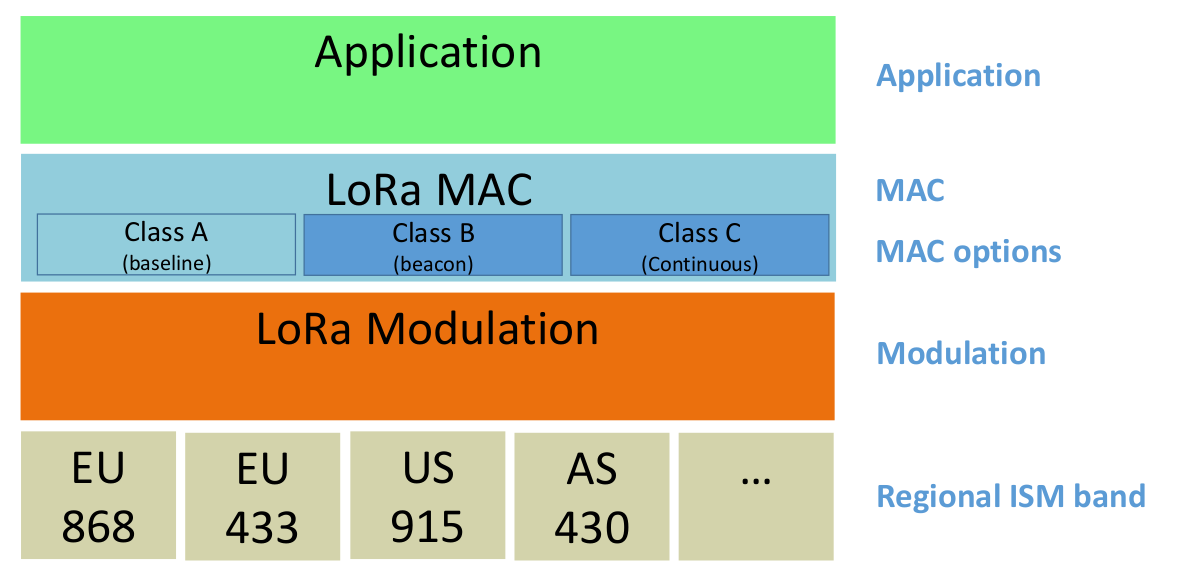
\includegraphics[width=1\textwidth]{Figures/node_architecture}        
            \caption{Architektura aplikace koncového zařízení}
            \label{fig:LoRaWAN_nodeswarch}
        \end{centering}
    \end{figure}

    Aplikaci zařízení, lze, z hlediska LoRaWAN, rozdělit do celkem 4 vrstev:

    \begin{description}
        \item [Aplikace] (Application) --- "uživatelský" program běžící na zařízení. Jeho
            zodpovědností je připravovat data zasílaná na aplikační server,
            popř. reagovat na přijaté požadavky. Pro samotné zasílání dat používá
            API LoRa MAC vrstvy (knihovny).
        \item [LoRa MAC] zodpovídá za vše co souvisí s LoRaWAN standardem. 
            Například aktivace, uchovávání informací souvisejících se spojením,
            zpracování MAC příkazů atp. Pro rádiovou komunikaci používá API
            nižší vrstvy, obvykle rádiového modulu. 
        \item [LoRa Modulation] (LoRa modulace) je obvykle prováděna přislušným
            rádiovým modulem. Jeho zodpovědností je odesílání a příjem LoRa 
            (popř. FSK) paketů. Obsah zpráv, použité frekvence, SF a CR hodnoty
            jsou dány vyšší vrstvou (LoRa MAC).
        \item [Regional ISM band] (regionální ISM pásmo) --- slouží jako médium
            pro bezdrátovou komunikaci. Jeho parametry musí být známy MAC vrstvě.
    \end{description}



\chapter{Popis technických vlastností a použití rozhraní NFC}
% Co to je, co s čím a jak komunikuje, normy, možnosti využití (?)

% Popis technických vlastností a použití rozhraní NFC.

% Jaké jsou NFC tagy?
% Jak se s nimi komunikuje? Jaké jsou tam příkazy?
% Něco k fungování mobilu samotného jako NFC tag
% Co je dynamický NFC tag
% Popis toho co použitý NFC tag umí a co neumí

%Vlastně můžu přepsat co jsem si zapsal --- moc víc toho není.

% Info zde je z doporučené knihy
\section{Obecný popis NFC}

    NFC je technologie umožňující bezdrátovou výměnu krátkých zpráv na 
    krátké vzdálenosti, typicky v jednotkách centimetrů.

    NFC vychází z RFID komunikace, konkrétně z normy ISO-14443 popisující
    komunikaci na frekvenci 13,56 MHz.

    Ačkoli jsou specifikace NFC dostupné (po zakoupení), je tato technologie 
    patentem, proto je nutno pro vývoj a výrobů zařízení tuto technologii 
    užívajících zakoupit příslušnou licenci.

    Komunikace probíhá mezi dvěma zařízeními, v jednom ze dvou režimů:

    \begin{description}
        \item [Aktivní] obě komunikující zařízení mají svůj vlastní zdroj
            energie (typicky baterii) --- například komunikace mezi dvěma mobilními telefony
        \item [Pasivní] jedno z komunikujících zařízení má vlastní zdroj energie
            a generuje rádiový signál, druhé je tímto signálem napájeno a
            odpovídá na zaslané požadavky.
    \end{description}

    Při komunikaci v pasivním režimu se zařízení napájené rádiovým polem obvykle
    označuje jako NFC tag. Tento režim je v kontextu používání mobilních 
    telefonů známější.

\section{Typy NFC tagů}

    Existují 4 typy NFC tagů standardizované NFC Fórem, a několik dalších typů
    definovaných jejich výrobci. Standardizované tagy jsou označeny jako 
    typ 1 až typ 4.

    Jednotlivé typy se navzájem liší zpravidla limity pro paměť, přenosovými 
    rychlostmi a podporovanými příkazy, podporou pro čtení či čtení i zápis a 
    dalšími vlastnostmi, např. možnostmi detekce kolizí při komunikaci.

\section{NDEF}

% TODO: Vzhledem k tomu že řeším parsování obsahu NDEF, bylo by vhodné
% zde jeho strukturu více rozepsat.

    Výrazným rozdílem oproti ostatním RFID technologiím je použití 
    standardizovaného datového formátu, --- NFC Data Exchange Format. Díky tomu
    může vývojář aplikace používající NFC přenechat řešení specifik různých
    typů tagů na použité knihovně, a pracovat pouze se zaslanými/přijatými daty,
    jejichž formát je známý.
    
    Základní jednotkou dat je NDEF Message (zpráva), která
    obsahuje jeden nebo více NFC Record ("záznam"). Tyto záznamy se skládají z
    hlavičky a samotných zasílaných dat.

    Hlavička záznamu obsahuje zejména informace o délce a typu dat v záznamu
    obsažených, navíc pak např. informace o tom, zda se jedná o první či o
    poslední záznam ve zprávě. 

    Z informací o typu (či formátu) dat je nejdůležitější pole označené jako 
    Payload Type, které obsahuje textový řetězec popisující formát dat. 
    Formát toho řetězce však závisí na 3 bitové hdnotě TNF 
    (Type Name Format), která může nabývat osmi hodnot:
    
    \begin{description}
        \item [0 --- Empty] Značí nepřítomnost dat, v tomto případě ani pole 
            Payload Type není přítomno
        \item [1 --- Well-known] Data jsou v jednom z formátů definovaných NFC
            fórem, například (v závorce odpovídající řetězec pole Payload Type)
            \begin{itemize}
                \item Prostý text, obsahující navíc informace o kódování a 
                    jazyce ("T")
                \item URI, tj. internetová adresa. Pro snížení množství dat jsou
                    však některé její části zakódovány dle NDEF standardů ("U")
                \item Smart Poster ("Sp")
            \end{itemize}
        \item [2 --- MIME media type] Například "text/json", "image/gif" atp.
        \item [3 --- Absolute URI] URI, odkazující na dokument popisující formát
            přenášených dat
        \item [4 --- External] Uživatelsky definovaný typ, například Android
            Application Record, obsahující informaci o tom jaká aplikace se má
            po načtení tagu spustit
        \item [5 --- Unknown] Pole Payload Type není přítomno
        \item [6 --- Unchanged] Stejný typ jako u předcházejícího záznamu --- 
            tento typ nemůže být u prvního záznamu ve zprávě
        \item [7 --- Reserved] Rezervováno pro budoucí užití
    \end{description}
    
    Samotná zpráva nemá žádnou hlavičku --- skládá se
    pouze ze záznamů zařazených za sebe, první a poslední záznam jsou pak označeny
    příslušnými bity ve svých hlavičkách, díky čemuž komunikující zařízení
    pozná (do jisté míry) celistvost zprávy.
    První záznam mívá zpravidla zvláštní význam; 
    například OS Android dle prvního záznamu rozhoduje, která z aplikací
    bude spuštěna pro zpracování dat z tagu.


\section{Dynamické NFC tagy}

    Dynamické NFC tagy se od běžných liší možností přistupovat do paměti i 
    jinými způsoby než jen NFC komunikací, a případně i obsah paměti měnit;
    např. v závislosti na zapsaných datech, externích událostech atp.
    Pro generování těchto dat pak bývají tyto tagy doplněny mikrokontrolérem.

    Dynamický NFC tag je použit v této práci.

    % V této práci je použit dynamický NFC tag M24ST od výrobce ST 
    % Microelectronics. Obsahuje EEPROM paměť velikosti 8192B, ke které je možno
    % kromě NFC rozhraní přistupovat skrze I2C sběrnici. Dále je vybaven 
    % digitálním výstupem, pomocí nějž lze detekovat probíhající bezdrátovou 
    % komunikaci.

\chapter{Návrh řešení}

\section{Scénář používání}

\section{d}

\chapter{MCU}

\input{Chapters/mcu}

\chapter{Periferní zařízení}

\input{Chapters/periferie}

\chapter{Software}

\input{Chapters/sw}

\chapter{Android aplikace}

\input{Chapters/android_app}

% Seznam literatury
\printbibliography[title={Literatura}, heading=bibintoc]

\end{document}
